\documentclass[1p]{elsarticle_modified}
%\bibliographystyle{elsarticle-num}

%\usepackage[colorlinks]{hyperref}
%\usepackage{abbrmath_seonhwa} %\Abb, \Ascr, \Acal ,\Abf, \Afrak
\usepackage{amsfonts}
\usepackage{amssymb}
\usepackage{amsmath}
\usepackage{amsthm}
\usepackage{scalefnt}
\usepackage{amsbsy}
\usepackage{kotex}
\usepackage{caption}
\usepackage{subfig}
\usepackage{color}
\usepackage{graphicx}
\usepackage{xcolor} %% white, black, red, green, blue, cyan, magenta, yellow
\usepackage{float}
\usepackage{setspace}
\usepackage{hyperref}

\usepackage{tikz}
\usetikzlibrary{arrows}

\usepackage{multirow}
\usepackage{array} % fixed length table
\usepackage{hhline}

%%%%%%%%%%%%%%%%%%%%%
\makeatletter
\renewcommand*\env@matrix[1][\arraystretch]{%
	\edef\arraystretch{#1}%
	\hskip -\arraycolsep
	\let\@ifnextchar\new@ifnextchar
	\array{*\c@MaxMatrixCols c}}
\makeatother %https://tex.stackexchange.com/questions/14071/how-can-i-increase-the-line-spacing-in-a-matrix
%%%%%%%%%%%%%%%

\usepackage[normalem]{ulem}

\newcommand{\msout}[1]{\ifmmode\text{\sout{\ensuremath{#1}}}\else\sout{#1}\fi}
%SOURCE: \msout is \stkout macro in https://tex.stackexchange.com/questions/20609/strikeout-in-math-mode

\newcommand{\cancel}[1]{
	\ifmmode
	{\color{red}\msout{#1}}
	\else
	{\color{red}\sout{#1}}
	\fi
}

\newcommand{\add}[1]{
	{\color{blue}\uwave{#1}}
}

\newcommand{\replace}[2]{
	\ifmmode
	{\color{red}\msout{#1}}{\color{blue}\uwave{#2}}
	\else
	{\color{red}\sout{#1}}{\color{blue}\uwave{#2}}
	\fi
}

\newcommand{\Sol}{\mathcal{S}} %segment
\newcommand{\D}{D} %diagram
\newcommand{\A}{\mathcal{A}} %arc


%%%%%%%%%%%%%%%%%%%%%%%%%%%%%5 test

\def\sl{\operatorname{\textup{SL}}(2,\Cbb)}
\def\psl{\operatorname{\textup{PSL}}(2,\Cbb)}
\def\quan{\mkern 1mu \triangleright \mkern 1mu}

\theoremstyle{definition}
\newtheorem{thm}{Theorem}[section]
\newtheorem{prop}[thm]{Proposition}
\newtheorem{lem}[thm]{Lemma}
\newtheorem{ques}[thm]{Question}
\newtheorem{cor}[thm]{Corollary}
\newtheorem{defn}[thm]{Definition}
\newtheorem{exam}[thm]{Example}
\newtheorem{rmk}[thm]{Remark}
\newtheorem{alg}[thm]{Algorithm}

\newcommand{\I}{\sqrt{-1}}
\begin{document}

%\begin{frontmatter}
%
%\title{Boundary parabolic representations of knots up to 8 crossings}
%
%%% Group authors per affiliation:
%\author{Yunhi Cho} 
%\address{Department of Mathematics, University of Seoul, Seoul, Korea}
%\ead{yhcho@uos.ac.kr}
%
%
%\author{Seonhwa Kim} %\fnref{s_kim}}
%\address{Center for Geometry and Physics, Institute for Basic Science, Pohang, 37673, Korea}
%\ead{ryeona17@ibs.re.kr}
%
%\author{Hyuk Kim}
%\address{Department of Mathematical Sciences, Seoul National University, Seoul 08826, Korea}
%\ead{hyukkim@snu.ac.kr}
%
%\author{Seokbeom Yoon}
%\address{Department of Mathematical Sciences, Seoul National University, Seoul, 08826,  Korea}
%\ead{sbyoon15@snu.ac.kr}
%
%\begin{abstract}
%We find all boundary parabolic representation of knots up to 8 crossings.
%
%\end{abstract}
%\begin{keyword}
%    \MSC[2010] 57M25 
%\end{keyword}
%
%\end{frontmatter}

%\linenumbers
%\tableofcontents
%
\newcommand\colored[1]{\textcolor{white}{\rule[-0.35ex]{0.8em}{1.4ex}}\kern-0.8em\color{red} #1}%
%\newcommand\colored[1]{\textcolor{white}{ #1}\kern-2.17ex	\textcolor{white}{ #1}\kern-1.81ex	\textcolor{white}{ #1}\kern-2.15ex\color{red}#1	}

{\Large $\underline{12a_{0436}~(K12a_{0436})}$}

\setlength{\tabcolsep}{10pt}
\renewcommand{\arraystretch}{1.6}
\vspace{1cm}\begin{tabular}{m{100pt}>{\centering\arraybackslash}m{274pt}}
\multirow{5}{120pt}{
	\centering
	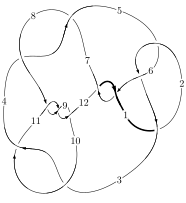
\includegraphics[width=112pt]{../../../GIT/diagram.site/Diagrams/png/1237_12a_0436.png}\\
\ \ \ A knot diagram\footnotemark}&
\allowdisplaybreaks
\textbf{Linearized knot diagam} \\
\cline{2-2}
 &
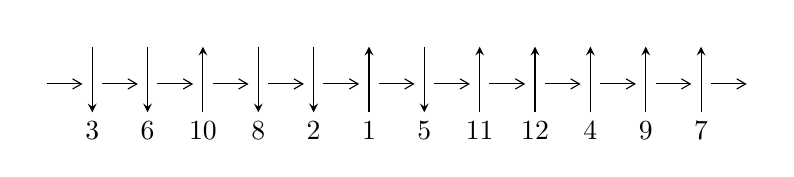
\begin{tikzpicture}[x=20pt, y=17pt]
	% nodes
	\node (C0) at (0, 0) {};
	\node (C1) at (1, 0) {};
	\node (C1U) at (1, +1) {};
	\node (C1D) at (1, -1) {3};

	\node (C2) at (2, 0) {};
	\node (C2U) at (2, +1) {};
	\node (C2D) at (2, -1) {6};

	\node (C3) at (3, 0) {};
	\node (C3U) at (3, +1) {};
	\node (C3D) at (3, -1) {10};

	\node (C4) at (4, 0) {};
	\node (C4U) at (4, +1) {};
	\node (C4D) at (4, -1) {8};

	\node (C5) at (5, 0) {};
	\node (C5U) at (5, +1) {};
	\node (C5D) at (5, -1) {2};

	\node (C6) at (6, 0) {};
	\node (C6U) at (6, +1) {};
	\node (C6D) at (6, -1) {1};

	\node (C7) at (7, 0) {};
	\node (C7U) at (7, +1) {};
	\node (C7D) at (7, -1) {5};

	\node (C8) at (8, 0) {};
	\node (C8U) at (8, +1) {};
	\node (C8D) at (8, -1) {11};

	\node (C9) at (9, 0) {};
	\node (C9U) at (9, +1) {};
	\node (C9D) at (9, -1) {12};

	\node (C10) at (10, 0) {};
	\node (C10U) at (10, +1) {};
	\node (C10D) at (10, -1) {4};

	\node (C11) at (11, 0) {};
	\node (C11U) at (11, +1) {};
	\node (C11D) at (11, -1) {9};

	\node (C12) at (12, 0) {};
	\node (C12U) at (12, +1) {};
	\node (C12D) at (12, -1) {7};
	\node (C13) at (13, 0) {};

	% arrows
	\draw[->,>={angle 60}]
	(C0) edge (C1) (C1) edge (C2) (C2) edge (C3) (C3) edge (C4) (C4) edge (C5) (C5) edge (C6) (C6) edge (C7) (C7) edge (C8) (C8) edge (C9) (C9) edge (C10) (C10) edge (C11) (C11) edge (C12) (C12) edge (C13) ;	\draw[->,>=stealth]
	(C1U) edge (C1D) (C2U) edge (C2D) (C3D) edge (C3U) (C4U) edge (C4D) (C5U) edge (C5D) (C6D) edge (C6U) (C7U) edge (C7D) (C8D) edge (C8U) (C9D) edge (C9U) (C10D) edge (C10U) (C11D) edge (C11U) (C12D) edge (C12U) ;
	\end{tikzpicture} \\
\hhline{~~} \\& 
\textbf{Solving Sequence} \\ \cline{2-2} 
 &
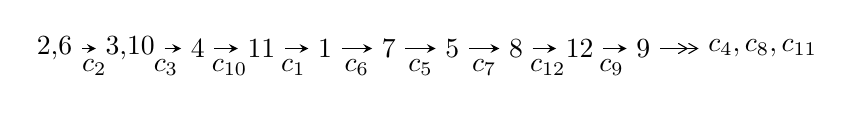
\begin{tikzpicture}[x=23pt, y=7pt]
	% node
	\node (A0) at (-1/8, 0) {2,6};
	\node (A1) at (17/16, 0) {3,10};
	\node (A2) at (17/8, 0) {4};
	\node (A3) at (25/8, 0) {11};
	\node (A4) at (33/8, 0) {1};
	\node (A5) at (41/8, 0) {7};
	\node (A6) at (49/8, 0) {5};
	\node (A7) at (57/8, 0) {8};
	\node (A8) at (65/8, 0) {12};
	\node (A9) at (73/8, 0) {9};
	\node (C1) at (1/2, -1) {$c_{2}$};
	\node (C2) at (13/8, -1) {$c_{3}$};
	\node (C3) at (21/8, -1) {$c_{10}$};
	\node (C4) at (29/8, -1) {$c_{1}$};
	\node (C5) at (37/8, -1) {$c_{6}$};
	\node (C6) at (45/8, -1) {$c_{5}$};
	\node (C7) at (53/8, -1) {$c_{7}$};
	\node (C8) at (61/8, -1) {$c_{12}$};
	\node (C9) at (69/8, -1) {$c_{9}$};
	\node (A10) at (11, 0) {$c_{4},c_{8},c_{11}$};

	% edge
	\draw[->,>=stealth]	
	(A0) edge (A1) (A1) edge (A2) (A2) edge (A3) (A3) edge (A4) (A4) edge (A5) (A5) edge (A6) (A6) edge (A7) (A7) edge (A8) (A8) edge (A9) ;
	\draw[->>,>={angle 60}]	
	(A9) edge (A10);
\end{tikzpicture} \\ 

\end{tabular} \\

\footnotetext{
The image of knot diagram is generated by the software ``\textbf{Draw programme}" developed by Andrew Bartholomew(\url{http://www.layer8.co.uk/maths/draw/index.htm\#Running-draw}), where we modified some parts for our purpose(\url{https://github.com/CATsTAILs/LinksPainter}).
}\phantom \\ \newline 
\centering \textbf{Ideals for irreducible components\footnotemark of $X_{\text{par}}$} 
 
\begin{align*}
I^u_{1}&=\langle 
-2 u^{79}+u^{78}+\cdots+b- u,\;- u^{78}- u^{77}+\cdots+a+3,\;u^{80}-2 u^{79}+\cdots- u-1\rangle \\
I^u_{2}&=\langle 
- u^6+2 u^4+u^3- u^2+b- u-1,\;- u^7- u^6+2 u^5+2 u^4- u^3- u^2+a- u-1,\\
\phantom{I^u_{2}}&\phantom{= \langle  }u^9+u^8-2 u^7-3 u^6+u^5+3 u^4+2 u^3- u-1\rangle \\
\\
\end{align*}
\raggedright * 2 irreducible components of $\dim_{\mathbb{C}}=0$, with total 89 representations.\\
\footnotetext{All coefficients of polynomials are rational numbers. But the coefficients are sometimes approximated in decimal forms when there is not enough margin.}
\newpage
\renewcommand{\arraystretch}{1}
\centering \section*{I. $I^u_{1}= \langle -2 u^{79}+u^{78}+\cdots+b- u,\;- u^{78}- u^{77}+\cdots+a+3,\;u^{80}-2 u^{79}+\cdots- u-1 \rangle$}
\flushleft \textbf{(i) Arc colorings}\\
\begin{tabular}{m{7pt} m{180pt} m{7pt} m{180pt} }
\flushright $a_{2}=$&$\begin{pmatrix}1\\0\end{pmatrix}$ \\
\flushright $a_{6}=$&$\begin{pmatrix}0\\u\end{pmatrix}$ \\
\flushright $a_{3}=$&$\begin{pmatrix}1\\u^2\end{pmatrix}$ \\
\flushright $a_{10}=$&$\begin{pmatrix}u^{78}+u^{77}+\cdots- u-3\\2 u^{79}- u^{78}+\cdots-4 u^2+u\end{pmatrix}$ \\
\flushright $a_{4}=$&$\begin{pmatrix}u^{17}-4 u^{15}+7 u^{13}-4 u^{11}-3 u^9+6 u^7-2 u^5+u\\u^{17}-5 u^{15}+11 u^{13}-12 u^{11}+5 u^9+2 u^7-2 u^5+u\end{pmatrix}$ \\
\flushright $a_{11}=$&$\begin{pmatrix}- u^{78}+u^{77}+\cdots+u-2\\- u^{78}+u^{77}+\cdots-2 u^3+2 u\end{pmatrix}$ \\
\flushright $a_{1}=$&$\begin{pmatrix}- u^2+1\\- u^4\end{pmatrix}$ \\
\flushright $a_{7}=$&$\begin{pmatrix}u^5-2 u^3+u\\u^7- u^5+u\end{pmatrix}$ \\
\flushright $a_{5}=$&$\begin{pmatrix}u\\u\end{pmatrix}$ \\
\flushright $a_{8}=$&$\begin{pmatrix}- u^9+2 u^7- u^5-2 u^3+u\\- u^9+3 u^7-3 u^5+u\end{pmatrix}$ \\
\flushright $a_{12}=$&$\begin{pmatrix}- u^8+3 u^6-3 u^4+1\\- u^{10}+2 u^8- u^6-2 u^4+u^2\end{pmatrix}$ \\
\flushright $a_{9}=$&$\begin{pmatrix}u^{77}- u^{76}+\cdots+2 u^2-2\\u^{79}- u^{78}+\cdots- u^2+2 u\end{pmatrix}$\\&\end{tabular}
\flushleft \textbf{(ii) Obstruction class $= -1$}\\~\\
\flushleft \textbf{(iii) Cusp Shapes $= -6 u^{79}+9 u^{78}+\cdots-29 u-1$}\\~\\
\newpage\renewcommand{\arraystretch}{1}
\flushleft \textbf{(iv) u-Polynomials at the component}\newline \\
\begin{tabular}{m{50pt}|m{274pt}}
Crossings & \hspace{64pt}u-Polynomials at each crossing \\
\hline $$\begin{aligned}c_{1}\end{aligned}$$&$\begin{aligned}
&u^{80}+42 u^{79}+\cdots+9 u+1
\end{aligned}$\\
\hline $$\begin{aligned}c_{2},c_{5}\end{aligned}$$&$\begin{aligned}
&u^{80}+2 u^{79}+\cdots+u-1
\end{aligned}$\\
\hline $$\begin{aligned}c_{3},c_{10}\end{aligned}$$&$\begin{aligned}
&u^{80}+u^{79}+\cdots-768 u^2+512
\end{aligned}$\\
\hline $$\begin{aligned}c_{4},c_{7}\end{aligned}$$&$\begin{aligned}
&u^{80}-6 u^{79}+\cdots+1829 u+145
\end{aligned}$\\
\hline $$\begin{aligned}c_{6},c_{12}\end{aligned}$$&$\begin{aligned}
&u^{80}+6 u^{79}+\cdots-577 u+53
\end{aligned}$\\
\hline $$\begin{aligned}c_{8},c_{9},c_{11}\end{aligned}$$&$\begin{aligned}
&u^{80}+10 u^{79}+\cdots-7 u-1
\end{aligned}$\\
\hline
\end{tabular}\\~\\
\newpage\renewcommand{\arraystretch}{1}
\flushleft \textbf{(v) Riley Polynomials at the component}\newline \\
\begin{tabular}{m{50pt}|m{274pt}}
Crossings & \hspace{64pt}Riley Polynomials at each crossing \\
\hline $$\begin{aligned}c_{1}\end{aligned}$$&$\begin{aligned}
&y^{80}-6 y^{79}+\cdots-41 y+1
\end{aligned}$\\
\hline $$\begin{aligned}c_{2},c_{5}\end{aligned}$$&$\begin{aligned}
&y^{80}-42 y^{79}+\cdots-9 y+1
\end{aligned}$\\
\hline $$\begin{aligned}c_{3},c_{10}\end{aligned}$$&$\begin{aligned}
&y^{80}-57 y^{79}+\cdots-786432 y+262144
\end{aligned}$\\
\hline $$\begin{aligned}c_{4},c_{7}\end{aligned}$$&$\begin{aligned}
&y^{80}+66 y^{79}+\cdots-1478221 y+21025
\end{aligned}$\\
\hline $$\begin{aligned}c_{6},c_{12}\end{aligned}$$&$\begin{aligned}
&y^{80}+54 y^{79}+\cdots-584997 y+2809
\end{aligned}$\\
\hline $$\begin{aligned}c_{8},c_{9},c_{11}\end{aligned}$$&$\begin{aligned}
&y^{80}-82 y^{79}+\cdots-5 y+1
\end{aligned}$\\
\hline
\end{tabular}\\~\\
\newpage\flushleft \textbf{(vi) Complex Volumes and Cusp Shapes}
$$\begin{array}{c|c|c}  
\text{Solutions to }I^u_{1}& \I (\text{vol} + \sqrt{-1}CS) & \text{Cusp shape}\\
 \hline 
\begin{aligned}
u &= \phantom{-}0.788241 + 0.593267 I \\
a &= \phantom{-}2.89714 + 1.16358 I \\
b &= \phantom{-}0.97355 + 2.78858 I\end{aligned}
 & \phantom{-}6.24334 - 5.11064 I & \phantom{-}8.14762 + 6.48257 I \\ \hline\begin{aligned}
u &= \phantom{-}0.788241 - 0.593267 I \\
a &= \phantom{-}2.89714 - 1.16358 I \\
b &= \phantom{-}0.97355 - 2.78858 I\end{aligned}
 & \phantom{-}6.24334 + 5.11064 I & \phantom{-}8.14762 - 6.48257 I \\ \hline\begin{aligned}
u &= \phantom{-}0.813592 + 0.609570 I \\
a &= -2.93002 - 1.26264 I \\
b &= -1.10331 - 2.68448 I\end{aligned}
 & \phantom{-}13.2744 - 9.2224 I & \phantom{-0.000000 } 0 \\ \hline\begin{aligned}
u &= \phantom{-}0.813592 - 0.609570 I \\
a &= -2.93002 + 1.26264 I \\
b &= -1.10331 + 2.68448 I\end{aligned}
 & \phantom{-}13.2744 + 9.2224 I & \phantom{-0.000000 } 0 \\ \hline\begin{aligned}
u &= -0.772569 + 0.598380 I \\
a &= \phantom{-}1.07413 + 1.28706 I \\
b &= \phantom{-}1.42261 + 0.64929 I\end{aligned}
 & \phantom{-}8.47306 + 2.34861 I & \phantom{-}9.12486 - 3.37977 I \\ \hline\begin{aligned}
u &= -0.772569 - 0.598380 I \\
a &= \phantom{-}1.07413 - 1.28706 I \\
b &= \phantom{-}1.42261 - 0.64929 I\end{aligned}
 & \phantom{-}8.47306 - 2.34861 I & \phantom{-}9.12486 + 3.37977 I \\ \hline\begin{aligned}
u &= \phantom{-}1.03436\phantom{ +0.000000I} \\
a &= \phantom{-}1.16159\phantom{ +0.000000I} \\
b &= \phantom{-}0.0399622\phantom{ +0.000000I}\end{aligned}
 & \phantom{-}3.30231\phantom{ +0.000000I} & \phantom{-0.000000 } 0 \\ \hline\begin{aligned}
u &= \phantom{-}0.755447 + 0.596084 I \\
a &= -2.64657 - 0.97416 I \\
b &= -0.97087 - 2.78244 I\end{aligned}
 & \phantom{-}6.33746 + 0.43474 I & \phantom{-}8.59846 + 0. I\phantom{ +0.000000I} \\ \hline\begin{aligned}
u &= \phantom{-}0.755447 - 0.596084 I \\
a &= -2.64657 + 0.97416 I \\
b &= -0.97087 + 2.78244 I\end{aligned}
 & \phantom{-}6.33746 - 0.43474 I & \phantom{-}8.59846 + 0. I\phantom{ +0.000000I} \\ \hline\begin{aligned}
u &= \phantom{-}0.731741 + 0.621831 I \\
a &= \phantom{-}2.26610 + 1.17730 I \\
b &= \phantom{-}0.78459 + 2.79549 I\end{aligned}
 & \phantom{-}13.5099 + 4.4268 I & \phantom{-}10.35839 + 0. I\phantom{ +0.000000I}\\
 \hline 
 \end{array}$$\newpage$$\begin{array}{c|c|c}  
\text{Solutions to }I^u_{1}& \I (\text{vol} + \sqrt{-1}CS) & \text{Cusp shape}\\
 \hline 
\begin{aligned}
u &= \phantom{-}0.731741 - 0.621831 I \\
a &= \phantom{-}2.26610 - 1.17730 I \\
b &= \phantom{-}0.78459 - 2.79549 I\end{aligned}
 & \phantom{-}13.5099 - 4.4268 I & \phantom{-}10.35839 + 0. I\phantom{ +0.000000I} \\ \hline\begin{aligned}
u &= -0.877134 + 0.339225 I \\
a &= \phantom{-}1.21807 - 1.37277 I \\
b &= \phantom{-}0.81822 - 1.38163 I\end{aligned}
 & \phantom{-}0.06759 + 3.08443 I & \phantom{-}2.43309 - 8.76495 I \\ \hline\begin{aligned}
u &= -0.877134 - 0.339225 I \\
a &= \phantom{-}1.21807 + 1.37277 I \\
b &= \phantom{-}0.81822 + 1.38163 I\end{aligned}
 & \phantom{-}0.06759 - 3.08443 I & \phantom{-}2.43309 + 8.76495 I \\ \hline\begin{aligned}
u &= -0.770687 + 0.535889 I \\
a &= -0.521106 - 0.626440 I \\
b &= -0.657130 - 0.323997 I\end{aligned}
 & \phantom{-}2.28869 + 2.16821 I & \phantom{-}1.72867 - 4.00408 I \\ \hline\begin{aligned}
u &= -0.770687 - 0.535889 I \\
a &= -0.521106 + 0.626440 I \\
b &= -0.657130 + 0.323997 I\end{aligned}
 & \phantom{-}2.28869 - 2.16821 I & \phantom{-}1.72867 + 4.00408 I \\ \hline\begin{aligned}
u &= -0.967844 + 0.492553 I \\
a &= -1.03957 + 1.74058 I \\
b &= -0.42685 + 2.01970 I\end{aligned}
 & \phantom{-}6.45001 + 4.97903 I & \phantom{-0.000000 } 0 \\ \hline\begin{aligned}
u &= -0.967844 - 0.492553 I \\
a &= -1.03957 - 1.74058 I \\
b &= -0.42685 - 2.01970 I\end{aligned}
 & \phantom{-}6.45001 - 4.97903 I & \phantom{-0.000000 } 0 \\ \hline\begin{aligned}
u &= \phantom{-}0.850210 + 0.090701 I \\
a &= -0.438624 - 0.409673 I \\
b &= \phantom{-}0.1052960 + 0.0201192 I\end{aligned}
 & -1.39732 - 0.27454 I & -6.35667 + 0.34095 I \\ \hline\begin{aligned}
u &= \phantom{-}0.850210 - 0.090701 I \\
a &= -0.438624 + 0.409673 I \\
b &= \phantom{-}0.1052960 - 0.0201192 I\end{aligned}
 & -1.39732 + 0.27454 I & -6.35667 - 0.34095 I \\ \hline\begin{aligned}
u &= -1.127480 + 0.258399 I \\
a &= -0.133039 + 1.121980 I \\
b &= -0.965050 + 0.962471 I\end{aligned}
 & \phantom{-}7.10133 + 5.72796 I & \phantom{-0.000000 } 0\\
 \hline 
 \end{array}$$\newpage$$\begin{array}{c|c|c}  
\text{Solutions to }I^u_{1}& \I (\text{vol} + \sqrt{-1}CS) & \text{Cusp shape}\\
 \hline 
\begin{aligned}
u &= -1.127480 - 0.258399 I \\
a &= -0.133039 - 1.121980 I \\
b &= -0.965050 - 0.962471 I\end{aligned}
 & \phantom{-}7.10133 - 5.72796 I & \phantom{-0.000000 } 0 \\ \hline\begin{aligned}
u &= \phantom{-}0.205648 + 0.805086 I \\
a &= -2.13997 + 0.84059 I \\
b &= -0.44039 - 1.84984 I\end{aligned}
 & \phantom{-}10.2271 + 10.5873 I & \phantom{-}8.12464 - 5.54004 I \\ \hline\begin{aligned}
u &= \phantom{-}0.205648 - 0.805086 I \\
a &= -2.13997 - 0.84059 I \\
b &= -0.44039 + 1.84984 I\end{aligned}
 & \phantom{-}10.2271 - 10.5873 I & \phantom{-}8.12464 + 5.54004 I \\ \hline\begin{aligned}
u &= \phantom{-}0.754822 + 0.340700 I \\
a &= \phantom{-}0.270589 + 1.097730 I \\
b &= -0.621443 - 0.083376 I\end{aligned}
 & \phantom{-}2.17846 - 1.57925 I & \phantom{-}3.82899 + 3.54363 I \\ \hline\begin{aligned}
u &= \phantom{-}0.754822 - 0.340700 I \\
a &= \phantom{-}0.270589 - 1.097730 I \\
b &= -0.621443 + 0.083376 I\end{aligned}
 & \phantom{-}2.17846 + 1.57925 I & \phantom{-}3.82899 - 3.54363 I \\ \hline\begin{aligned}
u &= -1.139280 + 0.328895 I \\
a &= \phantom{-}0.804519 - 0.439781 I \\
b &= \phantom{-}1.79318 - 1.05870 I\end{aligned}
 & -0.07200 + 2.42458 I & \phantom{-0.000000 } 0 \\ \hline\begin{aligned}
u &= -1.139280 - 0.328895 I \\
a &= \phantom{-}0.804519 + 0.439781 I \\
b &= \phantom{-}1.79318 + 1.05870 I\end{aligned}
 & -0.07200 - 2.42458 I & \phantom{-0.000000 } 0 \\ \hline\begin{aligned}
u &= \phantom{-}0.207211 + 0.779709 I \\
a &= \phantom{-}2.31171 - 0.83656 I \\
b &= \phantom{-}0.22750 + 1.53793 I\end{aligned}
 & \phantom{-}3.51520 + 6.34636 I & \phantom{-}6.24074 - 5.42401 I \\ \hline\begin{aligned}
u &= \phantom{-}0.207211 - 0.779709 I \\
a &= \phantom{-}2.31171 + 0.83656 I \\
b &= \phantom{-}0.22750 - 1.53793 I\end{aligned}
 & \phantom{-}3.51520 - 6.34636 I & \phantom{-}6.24074 + 5.42401 I \\ \hline\begin{aligned}
u &= -0.219389 + 0.769412 I \\
a &= \phantom{-}0.587178 - 0.807351 I \\
b &= -0.709890 - 1.068920 I\end{aligned}
 & \phantom{-}5.91566 - 3.66945 I & \phantom{-}7.65776 + 2.47936 I\\
 \hline 
 \end{array}$$\newpage$$\begin{array}{c|c|c}  
\text{Solutions to }I^u_{1}& \I (\text{vol} + \sqrt{-1}CS) & \text{Cusp shape}\\
 \hline 
\begin{aligned}
u &= -0.219389 - 0.769412 I \\
a &= \phantom{-}0.587178 + 0.807351 I \\
b &= -0.709890 + 1.068920 I\end{aligned}
 & \phantom{-}5.91566 + 3.66945 I & \phantom{-}7.65776 - 2.47936 I \\ \hline\begin{aligned}
u &= \phantom{-}0.272716 + 0.749664 I \\
a &= \phantom{-}2.07259 - 0.63049 I \\
b &= \phantom{-}0.774645 + 0.671760 I\end{aligned}
 & \phantom{-}11.39820 - 2.75257 I & \phantom{-}9.62649 + 1.18045 I \\ \hline\begin{aligned}
u &= \phantom{-}0.272716 - 0.749664 I \\
a &= \phantom{-}2.07259 + 0.63049 I \\
b &= \phantom{-}0.774645 - 0.671760 I\end{aligned}
 & \phantom{-}11.39820 + 2.75257 I & \phantom{-}9.62649 - 1.18045 I \\ \hline\begin{aligned}
u &= -0.079116 + 0.793763 I \\
a &= -0.273217 - 0.675415 I \\
b &= -1.057360 + 0.708134 I\end{aligned}
 & \phantom{-}2.72585 - 4.14449 I & \phantom{-}6.24638 + 3.84786 I \\ \hline\begin{aligned}
u &= -0.079116 - 0.793763 I \\
a &= -0.273217 + 0.675415 I \\
b &= -1.057360 - 0.708134 I\end{aligned}
 & \phantom{-}2.72585 + 4.14449 I & \phantom{-}6.24638 - 3.84786 I \\ \hline\begin{aligned}
u &= \phantom{-}1.163210 + 0.326788 I \\
a &= \phantom{-}0.185302 + 1.026710 I \\
b &= -0.411450 + 0.171697 I\end{aligned}
 & \phantom{-}1.76495 + 0.23636 I & \phantom{-0.000000 } 0 \\ \hline\begin{aligned}
u &= \phantom{-}1.163210 - 0.326788 I \\
a &= \phantom{-}0.185302 - 1.026710 I \\
b &= -0.411450 - 0.171697 I\end{aligned}
 & \phantom{-}1.76495 - 0.23636 I & \phantom{-0.000000 } 0 \\ \hline\begin{aligned}
u &= \phantom{-}0.226952 + 0.751765 I \\
a &= -2.32110 + 0.59136 I \\
b &= -0.256373 - 1.002050 I\end{aligned}
 & \phantom{-}3.98475 + 0.88483 I & \phantom{-}7.59092 + 0.37098 I \\ \hline\begin{aligned}
u &= \phantom{-}0.226952 - 0.751765 I \\
a &= -2.32110 - 0.59136 I \\
b &= -0.256373 + 1.002050 I\end{aligned}
 & \phantom{-}3.98475 - 0.88483 I & \phantom{-}7.59092 - 0.37098 I \\ \hline\begin{aligned}
u &= -1.177730 + 0.334016 I \\
a &= -0.472654 - 0.401659 I \\
b &= -2.13844 + 0.19517 I\end{aligned}
 & -0.65300 - 2.79770 I & \phantom{-0.000000 } 0\\
 \hline 
 \end{array}$$\newpage$$\begin{array}{c|c|c}  
\text{Solutions to }I^u_{1}& \I (\text{vol} + \sqrt{-1}CS) & \text{Cusp shape}\\
 \hline 
\begin{aligned}
u &= -1.177730 - 0.334016 I \\
a &= -0.472654 + 0.401659 I \\
b &= -2.13844 - 0.19517 I\end{aligned}
 & -0.65300 + 2.79770 I & \phantom{-0.000000 } 0 \\ \hline\begin{aligned}
u &= \phantom{-}1.167430 + 0.376595 I \\
a &= -0.002258 - 0.504828 I \\
b &= \phantom{-}0.295211 - 0.022642 I\end{aligned}
 & -3.96959 - 0.86076 I & \phantom{-0.000000 } 0 \\ \hline\begin{aligned}
u &= \phantom{-}1.167430 - 0.376595 I \\
a &= -0.002258 + 0.504828 I \\
b &= \phantom{-}0.295211 + 0.022642 I\end{aligned}
 & -3.96959 + 0.86076 I & \phantom{-0.000000 } 0 \\ \hline\begin{aligned}
u &= -1.150850 + 0.438169 I \\
a &= \phantom{-}1.26868 - 1.79458 I \\
b &= \phantom{-}0.29661 - 2.76608 I\end{aligned}
 & -2.44030 + 2.93931 I & \phantom{-0.000000 } 0 \\ \hline\begin{aligned}
u &= -1.150850 - 0.438169 I \\
a &= \phantom{-}1.26868 + 1.79458 I \\
b &= \phantom{-}0.29661 + 2.76608 I\end{aligned}
 & -2.44030 - 2.93931 I & \phantom{-0.000000 } 0 \\ \hline\begin{aligned}
u &= -0.166236 + 0.742708 I \\
a &= -0.347964 + 0.352578 I \\
b &= \phantom{-}0.365823 + 0.491960 I\end{aligned}
 & -0.13713 - 2.80838 I & -0.38510 + 3.25626 I \\ \hline\begin{aligned}
u &= -0.166236 - 0.742708 I \\
a &= -0.347964 - 0.352578 I \\
b &= \phantom{-}0.365823 - 0.491960 I\end{aligned}
 & -0.13713 + 2.80838 I & -0.38510 - 3.25626 I \\ \hline\begin{aligned}
u &= \phantom{-}1.154970 + 0.462037 I \\
a &= -0.067535 - 0.742060 I \\
b &= \phantom{-}1.304340 - 0.231466 I\end{aligned}
 & -2.26506 - 5.18346 I & \phantom{-0.000000 } 0 \\ \hline\begin{aligned}
u &= \phantom{-}1.154970 - 0.462037 I \\
a &= -0.067535 + 0.742060 I \\
b &= \phantom{-}1.304340 + 0.231466 I\end{aligned}
 & -2.26506 + 5.18346 I & \phantom{-0.000000 } 0 \\ \hline\begin{aligned}
u &= -1.199980 + 0.328265 I \\
a &= -0.111881 + 0.662316 I \\
b &= \phantom{-}1.80309 + 0.35042 I\end{aligned}
 & \phantom{-}5.92061 - 6.93082 I & \phantom{-0.000000 } 0\\
 \hline 
 \end{array}$$\newpage$$\begin{array}{c|c|c}  
\text{Solutions to }I^u_{1}& \I (\text{vol} + \sqrt{-1}CS) & \text{Cusp shape}\\
 \hline 
\begin{aligned}
u &= -1.199980 - 0.328265 I \\
a &= -0.111881 - 0.662316 I \\
b &= \phantom{-}1.80309 - 0.35042 I\end{aligned}
 & \phantom{-}5.92061 + 6.93082 I & \phantom{-0.000000 } 0 \\ \hline\begin{aligned}
u &= -0.491306 + 0.571190 I \\
a &= \phantom{-}1.91932 - 0.18659 I \\
b &= \phantom{-}1.09981 - 1.13296 I\end{aligned}
 & \phantom{-}7.80506 - 0.69666 I & \phantom{-}10.81571 + 0.01021 I \\ \hline\begin{aligned}
u &= -0.491306 - 0.571190 I \\
a &= \phantom{-}1.91932 + 0.18659 I \\
b &= \phantom{-}1.09981 + 1.13296 I\end{aligned}
 & \phantom{-}7.80506 + 0.69666 I & \phantom{-}10.81571 - 0.01021 I \\ \hline\begin{aligned}
u &= \phantom{-}1.175660 + 0.429014 I \\
a &= \phantom{-}0.607234 + 0.484749 I \\
b &= -0.402768 + 0.642166 I\end{aligned}
 & -5.55054 - 2.10141 I & \phantom{-0.000000 } 0 \\ \hline\begin{aligned}
u &= \phantom{-}1.175660 - 0.429014 I \\
a &= \phantom{-}0.607234 - 0.484749 I \\
b &= -0.402768 - 0.642166 I\end{aligned}
 & -5.55054 + 2.10141 I & \phantom{-0.000000 } 0 \\ \hline\begin{aligned}
u &= \phantom{-}1.138020 + 0.537928 I \\
a &= -0.45342 - 1.67252 I \\
b &= \phantom{-}0.04188 - 2.69443 I\end{aligned}
 & \phantom{-}8.86470 - 2.09320 I & \phantom{-0.000000 } 0 \\ \hline\begin{aligned}
u &= \phantom{-}1.138020 - 0.537928 I \\
a &= -0.45342 + 1.67252 I \\
b &= \phantom{-}0.04188 + 2.69443 I\end{aligned}
 & \phantom{-}8.86470 + 2.09320 I & \phantom{-0.000000 } 0 \\ \hline\begin{aligned}
u &= -1.175440 + 0.467052 I \\
a &= -0.49611 + 1.66574 I \\
b &= \phantom{-}0.51823 + 1.94433 I\end{aligned}
 & -5.28059 + 6.34553 I & \phantom{-0.000000 } 0 \\ \hline\begin{aligned}
u &= -1.175440 - 0.467052 I \\
a &= -0.49611 - 1.66574 I \\
b &= \phantom{-}0.51823 - 1.94433 I\end{aligned}
 & -5.28059 - 6.34553 I & \phantom{-0.000000 } 0 \\ \hline\begin{aligned}
u &= \phantom{-}1.155270 + 0.526476 I \\
a &= \phantom{-}1.25110 + 1.63810 I \\
b &= \phantom{-}0.59528 + 3.31320 I\end{aligned}
 & \phantom{-}1.27066 - 5.68261 I & \phantom{-0.000000 } 0\\
 \hline 
 \end{array}$$\newpage$$\begin{array}{c|c|c}  
\text{Solutions to }I^u_{1}& \I (\text{vol} + \sqrt{-1}CS) & \text{Cusp shape}\\
 \hline 
\begin{aligned}
u &= \phantom{-}1.155270 - 0.526476 I \\
a &= \phantom{-}1.25110 - 1.63810 I \\
b &= \phantom{-}0.59528 - 3.31320 I\end{aligned}
 & \phantom{-}1.27066 + 5.68261 I & \phantom{-0.000000 } 0 \\ \hline\begin{aligned}
u &= -1.168040 + 0.507921 I \\
a &= \phantom{-}0.922596 - 0.067964 I \\
b &= \phantom{-}0.845713 - 0.551844 I\end{aligned}
 & -3.04347 + 7.48824 I & \phantom{-0.000000 } 0 \\ \hline\begin{aligned}
u &= -1.168040 - 0.507921 I \\
a &= \phantom{-}0.922596 + 0.067964 I \\
b &= \phantom{-}0.845713 + 0.551844 I\end{aligned}
 & -3.04347 - 7.48824 I & \phantom{-0.000000 } 0 \\ \hline\begin{aligned}
u &= -0.052039 + 0.722252 I \\
a &= \phantom{-}0.562731 + 0.651978 I \\
b &= \phantom{-}0.444609 - 0.874281 I\end{aligned}
 & -2.07776 - 1.97235 I & -0.72819 + 4.37507 I \\ \hline\begin{aligned}
u &= -0.052039 - 0.722252 I \\
a &= \phantom{-}0.562731 - 0.651978 I \\
b &= \phantom{-}0.444609 + 0.874281 I\end{aligned}
 & -2.07776 + 1.97235 I & -0.72819 - 4.37507 I \\ \hline\begin{aligned}
u &= \phantom{-}1.207880 + 0.410981 I \\
a &= -1.070520 + 0.052109 I \\
b &= -0.330465 - 0.774725 I\end{aligned}
 & -1.086150 - 0.034868 I & \phantom{-0.000000 } 0 \\ \hline\begin{aligned}
u &= \phantom{-}1.207880 - 0.410981 I \\
a &= -1.070520 - 0.052109 I \\
b &= -0.330465 + 0.774725 I\end{aligned}
 & -1.086150 + 0.034868 I & \phantom{-0.000000 } 0 \\ \hline\begin{aligned}
u &= -1.162360 + 0.529806 I \\
a &= -1.79136 + 0.10388 I \\
b &= -1.64200 + 0.99199 I\end{aligned}
 & \phantom{-}3.15047 + 8.52143 I & \phantom{-0.000000 } 0 \\ \hline\begin{aligned}
u &= -1.162360 - 0.529806 I \\
a &= -1.79136 - 0.10388 I \\
b &= -1.64200 - 0.99199 I\end{aligned}
 & \phantom{-}3.15047 - 8.52143 I & \phantom{-0.000000 } 0 \\ \hline\begin{aligned}
u &= \phantom{-}1.168930 + 0.529133 I \\
a &= -1.57379 - 2.15421 I \\
b &= -0.32158 - 3.94599 I\end{aligned}
 & \phantom{-}0.69066 - 11.21750 I & \phantom{-0.000000 } 0\\
 \hline 
 \end{array}$$\newpage$$\begin{array}{c|c|c}  
\text{Solutions to }I^u_{1}& \I (\text{vol} + \sqrt{-1}CS) & \text{Cusp shape}\\
 \hline 
\begin{aligned}
u &= \phantom{-}1.168930 - 0.529133 I \\
a &= -1.57379 + 2.15421 I \\
b &= -0.32158 + 3.94599 I\end{aligned}
 & \phantom{-}0.69066 + 11.21750 I & \phantom{-0.000000 } 0 \\ \hline\begin{aligned}
u &= -1.198680 + 0.484977 I \\
a &= -0.36067 - 1.77130 I \\
b &= -1.37224 - 1.41960 I\end{aligned}
 & -0.56388 + 8.80154 I & \phantom{-0.000000 } 0 \\ \hline\begin{aligned}
u &= -1.198680 - 0.484977 I \\
a &= -0.36067 + 1.77130 I \\
b &= -1.37224 + 1.41960 I\end{aligned}
 & -0.56388 - 8.80154 I & \phantom{-0.000000 } 0 \\ \hline\begin{aligned}
u &= \phantom{-}1.177620 + 0.535604 I \\
a &= \phantom{-}1.54399 + 2.51779 I \\
b &= -0.02257 + 4.06707 I\end{aligned}
 & \phantom{-}7.3556 - 15.5480 I & \phantom{-0.000000 } 0 \\ \hline\begin{aligned}
u &= \phantom{-}1.177620 - 0.535604 I \\
a &= \phantom{-}1.54399 - 2.51779 I \\
b &= -0.02257 - 4.06707 I\end{aligned}
 & \phantom{-}7.3556 + 15.5480 I & \phantom{-0.000000 } 0 \\ \hline\begin{aligned}
u &= \phantom{-}0.051946 + 0.647928 I \\
a &= -1.20181 - 0.95038 I \\
b &= \phantom{-}0.032509 + 0.883301 I\end{aligned}
 & \phantom{-}0.779065 + 0.993473 I & \phantom{-}4.68420 + 0.71894 I \\ \hline\begin{aligned}
u &= \phantom{-}0.051946 - 0.647928 I \\
a &= -1.20181 + 0.95038 I \\
b &= \phantom{-}0.032509 - 0.883301 I\end{aligned}
 & \phantom{-}0.779065 - 0.993473 I & \phantom{-}4.68420 - 0.71894 I \\ \hline\begin{aligned}
u &= -0.543478 + 0.231554 I \\
a &= -2.18956 + 0.34629 I \\
b &= -1.118450 + 0.604202 I\end{aligned}
 & \phantom{-}1.049580 - 0.014357 I & \phantom{-}9.39150 - 0.35736 I \\ \hline\begin{aligned}
u &= -0.543478 - 0.231554 I \\
a &= -2.18956 - 0.34629 I \\
b &= -1.118450 - 0.604202 I\end{aligned}
 & \phantom{-}1.049580 + 0.014357 I & \phantom{-}9.39150 + 0.35736 I \\ \hline\begin{aligned}
u &= -0.490124\phantom{ +0.000000I} \\
a &= -2.52204\phantom{ +0.000000I} \\
b &= -1.18809\phantom{ +0.000000I}\end{aligned}
 & \phantom{-}1.02225\phantom{ +0.000000I} & \phantom{-}10.6740\phantom{ +0.000000I}\\
 \hline 
 \end{array}$$\newpage\newpage\renewcommand{\arraystretch}{1}
\centering \section*{II. $I^u_{2}= \langle - u^6+2 u^4+u^3- u^2+b- u-1,\;- u^7- u^6+2 u^5+2 u^4- u^3- u^2+a- u-1,\;u^9+u^8-2 u^7-3 u^6+u^5+3 u^4+2 u^3- u-1 \rangle$}
\flushleft \textbf{(i) Arc colorings}\\
\begin{tabular}{m{7pt} m{180pt} m{7pt} m{180pt} }
\flushright $a_{2}=$&$\begin{pmatrix}1\\0\end{pmatrix}$ \\
\flushright $a_{6}=$&$\begin{pmatrix}0\\u\end{pmatrix}$ \\
\flushright $a_{3}=$&$\begin{pmatrix}1\\u^2\end{pmatrix}$ \\
\flushright $a_{10}=$&$\begin{pmatrix}u^7+u^6-2 u^5-2 u^4+u^3+u^2+u+1\\u^6-2 u^4- u^3+u^2+u+1\end{pmatrix}$ \\
\flushright $a_{4}=$&$\begin{pmatrix}1\\u^2\end{pmatrix}$ \\
\flushright $a_{11}=$&$\begin{pmatrix}u^7+u^6-2 u^5-2 u^4+u^3+u^2+u+1\\u^6-2 u^4- u^3+u^2+u+1\end{pmatrix}$ \\
\flushright $a_{1}=$&$\begin{pmatrix}- u^2+1\\- u^4\end{pmatrix}$ \\
\flushright $a_{7}=$&$\begin{pmatrix}u^5-2 u^3+u\\u^7- u^5+u\end{pmatrix}$ \\
\flushright $a_{5}=$&$\begin{pmatrix}u\\u\end{pmatrix}$ \\
\flushright $a_{8}=$&$\begin{pmatrix}u^8-3 u^6+3 u^4-1\\u^8+u^7-3 u^6-2 u^5+3 u^4+2 u^3-1\end{pmatrix}$ \\
\flushright $a_{12}=$&$\begin{pmatrix}- u^8+3 u^6-3 u^4+1\\- u^8- u^7+3 u^6+2 u^5-3 u^4-2 u^3+1\end{pmatrix}$ \\
\flushright $a_{9}=$&$\begin{pmatrix}u^8+u^7-2 u^6-2 u^5+u^4+u^3+u^2+u\\u^8+u^7-2 u^6-2 u^5+u^4+u^3+u^2+u\end{pmatrix}$\\&\end{tabular}
\flushleft \textbf{(ii) Obstruction class $= 1$}\\~\\
\flushleft \textbf{(iii) Cusp Shapes $= - u^8-6 u^7+u^6+12 u^5+5 u^4-10 u^3-7 u^2-7 u+6$}\\~\\
\newpage\renewcommand{\arraystretch}{1}
\flushleft \textbf{(iv) u-Polynomials at the component}\newline \\
\begin{tabular}{m{50pt}|m{274pt}}
Crossings & \hspace{64pt}u-Polynomials at each crossing \\
\hline $$\begin{aligned}c_{1}\end{aligned}$$&$\begin{aligned}
&u^9-5 u^8+12 u^7-15 u^6+9 u^5+u^4-4 u^3+2 u^2+u-1
\end{aligned}$\\
\hline $$\begin{aligned}c_{2}\end{aligned}$$&$\begin{aligned}
&u^9+u^8-2 u^7-3 u^6+u^5+3 u^4+2 u^3- u-1
\end{aligned}$\\
\hline $$\begin{aligned}c_{3},c_{10}\end{aligned}$$&$\begin{aligned}
&u^9
\end{aligned}$\\
\hline $$\begin{aligned}c_{4}\end{aligned}$$&$\begin{aligned}
&u^9+u^8+2 u^7+u^6+3 u^5+u^4+2 u^3+u-1
\end{aligned}$\\
\hline $$\begin{aligned}c_{5}\end{aligned}$$&$\begin{aligned}
&u^9- u^8-2 u^7+3 u^6+u^5-3 u^4+2 u^3- u+1
\end{aligned}$\\
\hline $$\begin{aligned}c_{6}\end{aligned}$$&$\begin{aligned}
&u^9-3 u^8+8 u^7-13 u^6+17 u^5-17 u^4+12 u^3-6 u^2+u+1
\end{aligned}$\\
\hline $$\begin{aligned}c_{7}\end{aligned}$$&$\begin{aligned}
&u^9- u^8+2 u^7- u^6+3 u^5- u^4+2 u^3+u+1
\end{aligned}$\\
\hline $$\begin{aligned}c_{8},c_{9}\end{aligned}$$&$\begin{aligned}
&(u+1)^9
\end{aligned}$\\
\hline $$\begin{aligned}c_{11}\end{aligned}$$&$\begin{aligned}
&(u-1)^9
\end{aligned}$\\
\hline $$\begin{aligned}c_{12}\end{aligned}$$&$\begin{aligned}
&u^9+3 u^8+8 u^7+13 u^6+17 u^5+17 u^4+12 u^3+6 u^2+u-1
\end{aligned}$\\
\hline
\end{tabular}\\~\\
\newpage\renewcommand{\arraystretch}{1}
\flushleft \textbf{(v) Riley Polynomials at the component}\newline \\
\begin{tabular}{m{50pt}|m{274pt}}
Crossings & \hspace{64pt}Riley Polynomials at each crossing \\
\hline $$\begin{aligned}c_{1}\end{aligned}$$&$\begin{aligned}
&y^9- y^8+12 y^7-7 y^6+37 y^5+y^4-10 y^2+5 y-1
\end{aligned}$\\
\hline $$\begin{aligned}c_{2},c_{5}\end{aligned}$$&$\begin{aligned}
&y^9-5 y^8+12 y^7-15 y^6+9 y^5+y^4-4 y^3+2 y^2+y-1
\end{aligned}$\\
\hline $$\begin{aligned}c_{3},c_{10}\end{aligned}$$&$\begin{aligned}
&y^9
\end{aligned}$\\
\hline $$\begin{aligned}c_{4},c_{7}\end{aligned}$$&$\begin{aligned}
&y^9+3 y^8+8 y^7+13 y^6+17 y^5+17 y^4+12 y^3+6 y^2+y-1
\end{aligned}$\\
\hline $$\begin{aligned}c_{6},c_{12}\end{aligned}$$&$\begin{aligned}
&y^9+7 y^8+20 y^7+25 y^6+5 y^5-15 y^4+22 y^2+13 y-1
\end{aligned}$\\
\hline $$\begin{aligned}c_{8},c_{9},c_{11}\end{aligned}$$&$\begin{aligned}
&(y-1)^9
\end{aligned}$\\
\hline
\end{tabular}\\~\\
\newpage\flushleft \textbf{(vi) Complex Volumes and Cusp Shapes}
$$\begin{array}{c|c|c}  
\text{Solutions to }I^u_{2}& \I (\text{vol} + \sqrt{-1}CS) & \text{Cusp shape}\\
 \hline 
\begin{aligned}
u &= -0.772920 + 0.510351 I \\
a &= \phantom{-}0.147032 + 1.012940 I \\
b &= \phantom{-}0.848670 + 0.225310 I\end{aligned}
 & \phantom{-}3.42837 + 2.09337 I & \phantom{-}10.43453 - 4.18932 I \\ \hline\begin{aligned}
u &= -0.772920 - 0.510351 I \\
a &= \phantom{-}0.147032 - 1.012940 I \\
b &= \phantom{-}0.848670 - 0.225310 I\end{aligned}
 & \phantom{-}3.42837 - 2.09337 I & \phantom{-}10.43453 + 4.18932 I \\ \hline\begin{aligned}
u &= \phantom{-}0.825933\phantom{ +0.000000I} \\
a &= \phantom{-}1.95176\phantom{ +0.000000I} \\
b &= \phantom{-}1.33142\phantom{ +0.000000I}\end{aligned}
 & \phantom{-}0.446489\phantom{ +0.000000I} & -4.72420\phantom{ +0.000000I} \\ \hline\begin{aligned}
u &= \phantom{-}1.173910 + 0.391555 I \\
a &= -0.679689 - 0.626017 I \\
b &= -0.25695 - 1.39155 I\end{aligned}
 & -2.72642 - 1.33617 I & \phantom{-}0.549708 + 1.017936 I \\ \hline\begin{aligned}
u &= \phantom{-}1.173910 - 0.391555 I \\
a &= -0.679689 + 0.626017 I \\
b &= -0.25695 + 1.39155 I\end{aligned}
 & -2.72642 + 1.33617 I & \phantom{-}0.549708 - 1.017936 I \\ \hline\begin{aligned}
u &= -0.141484 + 0.739668 I \\
a &= \phantom{-}0.541407 - 0.753907 I \\
b &= -0.443165 + 0.284059 I\end{aligned}
 & \phantom{-}1.02799 - 2.45442 I & \phantom{-}6.31821 + 2.62939 I \\ \hline\begin{aligned}
u &= -0.141484 - 0.739668 I \\
a &= \phantom{-}0.541407 + 0.753907 I \\
b &= -0.443165 - 0.284059 I\end{aligned}
 & \phantom{-}1.02799 + 2.45442 I & \phantom{-}6.31821 - 2.62939 I \\ \hline\begin{aligned}
u &= -1.172470 + 0.500383 I \\
a &= -0.484630 - 0.655708 I \\
b &= -1.314260 - 0.168567 I\end{aligned}
 & -1.95319 + 7.08493 I & \phantom{-}3.05967 - 5.11095 I \\ \hline\begin{aligned}
u &= -1.172470 - 0.500383 I \\
a &= -0.484630 + 0.655708 I \\
b &= -1.314260 + 0.168567 I\end{aligned}
 & -1.95319 - 7.08493 I & \phantom{-}3.05967 + 5.11095 I\\
 \hline 
 \end{array}$$\newpage
\newpage\renewcommand{\arraystretch}{1}
\centering \section*{ III. u-Polynomials}
\begin{tabular}{m{50pt}|m{274pt}}
Crossings & \hspace{64pt}u-Polynomials at each crossing \\
\hline $$\begin{aligned}c_{1}\end{aligned}$$&$\begin{aligned}
&(u^9-5 u^8+12 u^7-15 u^6+9 u^5+u^4-4 u^3+2 u^2+u-1)\\
&\cdot(u^{80}+42 u^{79}+\cdots+9 u+1)
\end{aligned}$\\
\hline $$\begin{aligned}c_{2}\end{aligned}$$&$\begin{aligned}
&(u^9+u^8+\cdots- u-1)(u^{80}+2 u^{79}+\cdots+u-1)
\end{aligned}$\\
\hline $$\begin{aligned}c_{3},c_{10}\end{aligned}$$&$\begin{aligned}
&u^9(u^{80}+u^{79}+\cdots-768 u^2+512)
\end{aligned}$\\
\hline $$\begin{aligned}c_{4}\end{aligned}$$&$\begin{aligned}
&(u^9+u^8+2 u^7+u^6+3 u^5+u^4+2 u^3+u-1)\\
&\cdot(u^{80}-6 u^{79}+\cdots+1829 u+145)
\end{aligned}$\\
\hline $$\begin{aligned}c_{5}\end{aligned}$$&$\begin{aligned}
&(u^9- u^8+\cdots- u+1)(u^{80}+2 u^{79}+\cdots+u-1)
\end{aligned}$\\
\hline $$\begin{aligned}c_{6}\end{aligned}$$&$\begin{aligned}
&(u^9-3 u^8+8 u^7-13 u^6+17 u^5-17 u^4+12 u^3-6 u^2+u+1)\\
&\cdot(u^{80}+6 u^{79}+\cdots-577 u+53)
\end{aligned}$\\
\hline $$\begin{aligned}c_{7}\end{aligned}$$&$\begin{aligned}
&(u^9- u^8+2 u^7- u^6+3 u^5- u^4+2 u^3+u+1)\\
&\cdot(u^{80}-6 u^{79}+\cdots+1829 u+145)
\end{aligned}$\\
\hline $$\begin{aligned}c_{8},c_{9}\end{aligned}$$&$\begin{aligned}
&((u+1)^9)(u^{80}+10 u^{79}+\cdots-7 u-1)
\end{aligned}$\\
\hline $$\begin{aligned}c_{11}\end{aligned}$$&$\begin{aligned}
&((u-1)^9)(u^{80}+10 u^{79}+\cdots-7 u-1)
\end{aligned}$\\
\hline $$\begin{aligned}c_{12}\end{aligned}$$&$\begin{aligned}
&(u^9+3 u^8+8 u^7+13 u^6+17 u^5+17 u^4+12 u^3+6 u^2+u-1)\\
&\cdot(u^{80}+6 u^{79}+\cdots-577 u+53)
\end{aligned}$\\
\hline
\end{tabular}\newpage\renewcommand{\arraystretch}{1}
\centering \section*{ IV. Riley Polynomials}
\begin{tabular}{m{50pt}|m{274pt}}
Crossings & \hspace{64pt}Riley Polynomials at each crossing \\
\hline $$\begin{aligned}c_{1}\end{aligned}$$&$\begin{aligned}
&(y^9- y^8+12 y^7-7 y^6+37 y^5+y^4-10 y^2+5 y-1)\\
&\cdot(y^{80}-6 y^{79}+\cdots-41 y+1)
\end{aligned}$\\
\hline $$\begin{aligned}c_{2},c_{5}\end{aligned}$$&$\begin{aligned}
&(y^9-5 y^8+12 y^7-15 y^6+9 y^5+y^4-4 y^3+2 y^2+y-1)\\
&\cdot(y^{80}-42 y^{79}+\cdots-9 y+1)
\end{aligned}$\\
\hline $$\begin{aligned}c_{3},c_{10}\end{aligned}$$&$\begin{aligned}
&y^9(y^{80}-57 y^{79}+\cdots-786432 y+262144)
\end{aligned}$\\
\hline $$\begin{aligned}c_{4},c_{7}\end{aligned}$$&$\begin{aligned}
&(y^9+3 y^8+8 y^7+13 y^6+17 y^5+17 y^4+12 y^3+6 y^2+y-1)\\
&\cdot(y^{80}+66 y^{79}+\cdots-1478221 y+21025)
\end{aligned}$\\
\hline $$\begin{aligned}c_{6},c_{12}\end{aligned}$$&$\begin{aligned}
&(y^9+7 y^8+20 y^7+25 y^6+5 y^5-15 y^4+22 y^2+13 y-1)\\
&\cdot(y^{80}+54 y^{79}+\cdots-584997 y+2809)
\end{aligned}$\\
\hline $$\begin{aligned}c_{8},c_{9},c_{11}\end{aligned}$$&$\begin{aligned}
&((y-1)^9)(y^{80}-82 y^{79}+\cdots-5 y+1)
\end{aligned}$\\
\hline
\end{tabular}
\vskip 2pc
\end{document}